%%%%%%%%%%%%%%%%%%%%%%%%%%%%%%%%%%%%%%%

\chapter{~~Description de la génération de colonnes \label{gencol}}

\section{Introduction}


La génération de colonnes permet de résoudre des PLNE de grandes tailles. Cette méthode est souvent utilisée pour les problèmes de \vrptw (cf. \cite{feillet2010}). Comme notre problème est très proche, on peut espérer que cette méthode nous apportera de bons résultats. 

Le principe général de la génération de colonnes \cite{barnhart1998branch,feillet2010} est le suivant : on décompose le problème en deux problèmes, un Problème Maître (Master Problem en anglais, noté MP) et un sous-problème (Pricing Sub-Problem  en anglais, noté PSP).
Le PSP trouve des "colonnes" améliorantes et les ajoute au MP.
Toute solution du PSP forme une solution du problème global. 
Par exemple, pour notre problème, une solution du PSP est une tournée pour un technicien. 
Cette route forme bien une solution du problème, même si elle n'est clairement pas optimale.

Le MP calcule une solution optimale avec l'ajout de ces colonnes. 
Puis il fournit au PSP les coûts réduits (cf. Définition~\ref{def:cout}) pour qu'il trouve de nouvelles colonnes.
On répète ce mécanisme tant que le PSP trouve des colonnes améliorantes (cf Figure~\ref{fig:gencol}).

Il existe plusieurs types de décomposition comme par exemple la décomposition de Dantzig-Wolfe \cite{dantzig1960decomposition} ou la décomposition de Benders \cite{benders1962partitioning}, ces décompositions s'appuient sur la structure de la matrice du programme linéaire associé. Ces décompositions influencent le modèle MP et la structure du PSP.

\begin{figure}[H]
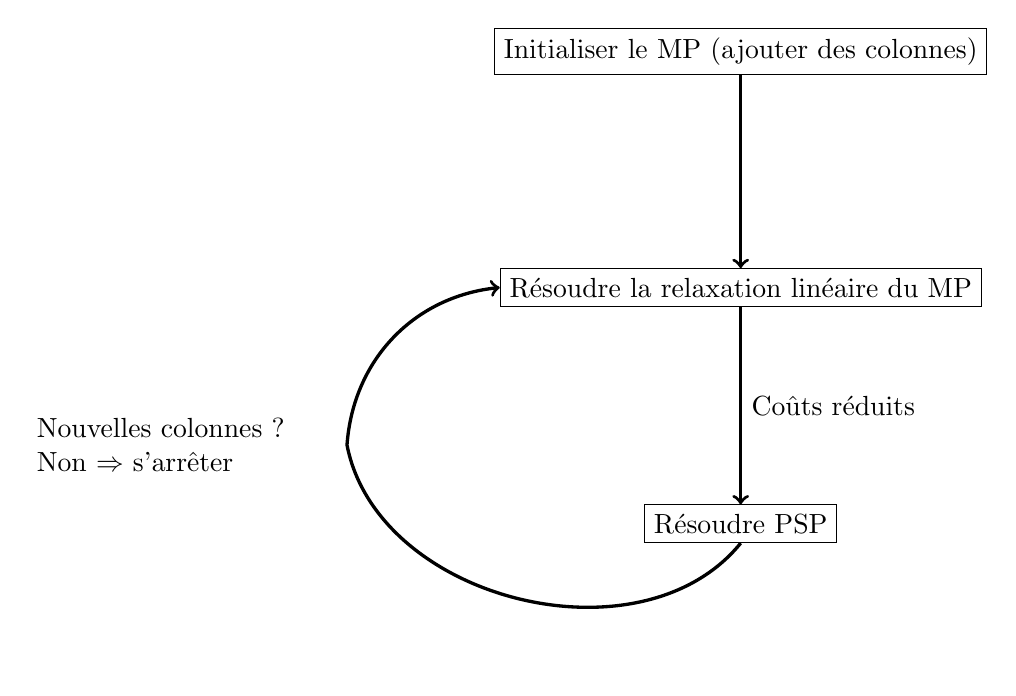
\begin{tikzpicture}

\node[draw,rectangle] (0) at (5,5) {Initialiser le MP (ajouter des colonnes)};
\node[draw,rectangle] (1) at (5,2) {Résoudre la relaxation linéaire du MP};
\node[draw,rectangle] (2) at (5,-1) {Résoudre PSP};

\draw[->,very thick] (0)--(1);
\draw[->,very thick] (1)--(2)node[right,midway]{Coûts réduits};
\draw[->,very thick] (2.south) to[bend left=65] (0,0) to[bend left=40](1.west)node[left,midway,text width = 3.8cm]{Nouvelles colonnes ? Non $\Rightarrow$ s'arrêter};
\end{tikzpicture}
\caption{Schéma général de la génération de colonnes \label{fig:gencol}}
\end{figure}

%Pour passer de la formulation générale \ref{MIP:Model1} vers un problème de génération de colonnes nous devons changer la modélisation initiale.
Actuellement nous créons chaque tournée de techniciens dans le même problème.
Nous définissons donc un problème permettant de créer une tournée pour un technicien donné (PSP) et un problème permettant d'optimiser l'ensemble des tournées de techniciens (MP).
Le MP résout le problème dans sa globalité alors que le PSP résout le problème localement, pour un seul technicien à la fois. Chaque solution du PSP nous donne une tournée réalisable pour un technicien, c'est-à-dire que cette tournée respecte toutes les contraintes de la formulation générale.
Le MP veille à ce que chaque tâche ne soit affectée qu'une seule fois, et que chaque technicien ne puisse faire au plus qu'une seule tournée. Il vérifie aussi les contraintes de précédences entre les tâches et les contraintes de même technicien.
Toute solution du MP représente bien une solution de la formulation générale car chacune des tournées est une tournée réalisable.

Dans la Section~\ref{sec:CG_illus} nous présentons un exemple illustratif pour expliquer l'intuition générale de la génération de colonnes puis dans la Section~\ref{sec:CG_RMP} nous expliquerons comment fonctionne le MP pour notre problème et dans la Section~\ref{sec:CG_PSP} nous détaillerons le comportement du PSP. 



%%%%%%%%%%%%%%%%%%%%%%%%%%%%%%%%%%%%%%%
%%%%%%%%%%%%%%%%%%%%%%%%%%%%%%%%%%%%%%%

\section{Illustration \label{sec:CG_illus}}
Dans cette section, nous présentons un exemple pour illustrer la génération de colonnes. 
Cet exemple, basé sur le problème de découpage ou Cutstock Problem en anglais a été identifié par Kantorovich et al.\cite{kantorovich1960mathematical}. 
Ensuite Gilmore et Gomory \cite{gilmore1961linear} proposent un algorithme utilisant la génération de colonnes pour résoudre le problème.
Le problème de découpage est $\np$-complet, notamment  par réduction du problème du sac à dos \cite{Karp1972}.

Le problème de découpage consiste à découper, dans des barres de taille fixe (disponibles en quantité infinie), des morceaux (appelés bobines) de tailles variables tout en minimisant le nombre total de barres utilisées.
Étant donné $\mathcal{W}$ la taille de la barre, on souhaite avoir $n$ bobines de taille $w_1$,$\ldots$,$w_n$ en quantité $d_1$,$\ldots$,$d_n$ avec $ w_i < \mathcal{W}~ \forall ~ i $.
Le but est donc de trouver des plans de découpe (cf. figure~\ref{fig:pattern}) pour obtenir toutes les bobines demandées en minimisant le nombre de barres utilisées.

\begin{figure}[H]
\centering
\begin{tikzpicture}

\node[] (14) at (-1,0.5) {$\rightarrow$};
\node[] (17) at (-3,0.5) {Plan de découpe 1};
\node[] (14) at (-1,-1.5) {$\rightarrow$};
\node[] (17) at (-3,-1.5) {bobines};

\node[] (0) at (0,0) {};
\node[] (1) at (0,1) {};
\draw[] (0.center) to[bend left](1.center);

\node[] (20) at (3,0) {};
\node[] (21) at (3,1) {};
\draw[dashed,thick] (20.center) to[bend left](21.center);

\node[] (30) at (7,0) {};
\node[] (31) at (7,1) {};
\draw[dashed,thick] (30.center) to[bend left](31.center);

\node[] (2) at (8,0) {};
\node[] (3) at (8,1) {};
\draw[] (2.center) to[bend left](3.center);
\draw[] (2.center) to[bend right](3.center);

\draw[] (0.center)--(2.center);
\draw[] (1.center)--(3.center);

\node[] (15) at (4,1.8) {Barre de taille fixe $k$};

\draw[decoration={brace,raise = 2pt,amplitude=10pt},decorate]
  (1.center)--(3.center);
  
\fill [pattern=horizontal lines] (30.center) to[bend left] (31.center) -- (3.center) to[bend right] (2.center);

\draw[decoration={brace,mirror,raise = 3pt,amplitude=5pt},decorate]
  (30.center)--(2.center);
\node[] (25) at (7.5,-0.5) {perte} ; 


\node[] (40) at (0,-2) {};
\node[] (41) at (0,-1) {};
\draw[] (40.center) to[bend left](41.center);

\node[] (50) at (3,-2) {};
\node[] (51) at (3,-1) {};
\draw[] (50.center) to[bend left](51.center);
\draw[] (50.center) to[bend right](51.center);
\draw[] (50.center)--(40.center);
\draw[] (51.center)--(41.center);

\node[] (140) at (4,-2) {};
\node[] (141) at (4,-1) {};
\draw[] (140.center) to[bend left](141.center);

\node[] (150) at (8,-2) {};
\node[] (151) at (8,-1) {};
\draw[] (150.center) to[bend left](151.center);
\draw[] (150.center) to[bend right](151.center);
\draw[] (150.center)--(140.center);
\draw[] (151.center)--(141.center);

\end{tikzpicture}
\caption{Schéma expliquant le principe d'un plan de découpe \label{fig:pattern}}
\end{figure}

Ce problème est très intéressant pour introduire la génération de colonnes car la formulation l'utilisant, cf. Table~\ref{table:RMP}, est plus naturelle que la formulation générale voir Table~\ref{table:general}.

\subsection{Formulation générale}

Pour la formulation générale, $y_k$ représente la barre $k$, et $y_k=1$ si la barre $k$ est utilisée. 
$x_{i}^k = $ nombre de fois où la bobine $i$ appartient au découpage de la barre $k$.
$\omega_i = $ à la taille de bobine $i$ et $\mathcal{W} = $ à la taille de la barre et $K = \sum\limits_{i=0}^n d_i$ représente le nombre maximal de barres que l'on peut utiliser. Au pire on utilise une barre où l'on découpe une bobine dedans, donc on utiliserait autant de barres que la somme des demandes de chaque bobine. 
Par exemple si on doit découper dans une barre deux bobines en quantité 10 et 20, $K=30$ : dans le pire des cas on utilise une barre pour découper chaque bobine.
Les contraintes \eqref{cut:gen:decoupage} permettent de gérer les découpages de la barre, autrement dit on découpe des bobines dans la barre tant que l'on ne dépasse pas la taille de la barre.
$K$ est une borne supérieure sur le nombre de barres utilisées.
De plus on crée les découpages à la volée ; c'est l'exécution du simplexe sur notre programme linéaire qui va nous dire quels sont les découpages des barres nécessaires pour obtenir la bonne quantité de chacune des bobines, cf. Contraintes~\eqref{cut:gen:bobine}.
On remarque que dans cette formulation il y a un très grand nombre de variables et de contraintes en fonction du nombre de barres disponibles.


\begin{table}[H]
\begin{align}%{*9l}
\text{Minimiser} &\sum\limits_{k=0}^K y_k \\ 
S.c. & \sum\limits_{k=0}^K  x_{i}^k \geq  d_i &&\forall i \in [1..m]\label{cut:gen:bobine}\\
& \sum\limits_{i=0}^m \omega_i  x_{i}^k  \leq  \mathcal{W}. ~ y_k   &&\forall k \in [1..K]\label{cut:gen:decoupage}\\
&  x_i^k \in \mathbb{N} && \forall k \in [1..K],~\forall i \in [1..m]\\
&  y_k \in \{0,1\} && \forall k \in [1..K]
\end{align}
\caption{Formulation générale du cut stock problem. \label{table:general}}
\end{table}

\subsection{Modèles et intérêts de la génération de colonnes}
Pour la formulation du Problème Maître \ref{table:RMP}, les variables de décisions $\lambda^p$ représentent le nombre de fois où le plan de découpage $p$ est utilisé, $a_{i}^p$ indique le nombre d’occurrence de la bobine $i$ dans le plan de découpe $p$.
Les contraintes \eqref{cut:general:demand} assurent que chacune des bobines est au moins découpée le bon nombre de fois. 
Pour écrire le programme linéaire il faut supposer que l'on possède tous les plans de découpages de la barre possibles, notons $\Omega$ l'ensemble des plans de découpages possibles, la taille de cet ensemble croit exponentiellement en fonction de la taille de la barre et des bobines.


\begin{table}[H]
\begin{align}
\text{Minimiser} &\sum\limits_{p\in \Omega}  ~ \lambda^p  \label{cut:general:obj}&&\\ 
S.c. & \sum\limits_{p\in\Omega}  a_{i}^p\lambda^{p} \geq d_i  && \forall i \in [1..m] \label{cut:general:demand}\\
& \lambda^k  \in \mathbb{N} && \forall p \in \Omega
\end{align}
\caption{Formulation du Problème Maître du cut stock problem. \label{table:RMP}}
\end{table}



Au lieu de créer l'ensemble des plans de découpage possibles, on utilise seulement un nombre restreint de plans de découpages, puis on ajoutera uniquement les plans de découpage améliorants grâce à un sous-problème.
Ce sous-problème consiste donc à trouver un plan de découpage améliorant : trouver une nouvelle affectation des bobines sur la barre pour obtenir un meilleur découpage (moins de pertes).
Une affectation des bobines sur la barre consiste à associer une valeur à chaque bobine, cette valeur indiquant le nombre d'occurrence découpée de cette bobine dans la barre.
Cependant il ne faut pas que cette affectation dépasse la taille de la barre.



Considérons l'exemple suivant : \\
Le tableau \ref{table:cutstock} représente les données de l'exemple.
\begin{table}[H]
\centering
\begin{tabular}{|l|l|l|}
\hline
 & taille & quantité\\
\hline
barre & 85 & $\infty$\\
bobine 1 & 25 & 50\\
bobine 2 & 40 & 36\\
bobine 3& 50 &24\\
\hline
\end{tabular}
\caption{Tableau récapitulant les tailles et quantités demandées de la barre et des bobines.\label{table:cutstock}}
\end{table}


Pour commencer le processus de génération de colonnes on définit trois plans de découpes : pour chaque bobine on coupe la barre en fonction du nombre maximal de fois où la bobine rentre dans la barre.
Par exemple on peut couper au plus trois fois la bobine 1 dans la barre ($3 * 25 = 75 < 85 $),  au plus deux fois la bobine 2 dans la barre ($2 * 40 = 80 < 85 $) et au plus une fois la bobine 3 dans la barre ($1 * 50 = 50 < 85 $) .
Ainsi une colonne représente un plan de découpe comme on peut le voir dans le programme linéaire \ref{table:lin1}.




Soit $x_1$ (resp. $x_2$ et resp. $x_3$) le nombre de barres utilisant le plan de découpe 1 (resp. 2 et resp. 3). Le programme linéaire suivant correspond au Programme Maître Restreint que nous définirons plus tard. 
Le programme doit sélectionner parmi un ensemble de plans de découpes, les meilleurs plans afin d'obtenir les bobines demandées.
Ici on n'a pas le choix, on doit utiliser le seul plan de découpe disponible pour chaque bobine pour obtenir la bonne quantité de chaque bobine.
Les contraintes de la Table~\ref{table:lin1} assurent que l'on fournit au moins la quantité demandée pour chacune des bobines.  
\begin{table}[H]

\centering
\begin{minipage}[t]{0.4\linewidth}
$$
\arraycolsep=2pt
\begin{array}{*8l}
\text{Minimiser} & x_1 & + & x_2 & + & x_3 & &\\
& 3~x_1 & & & & & \geq & 50\\
& & & 2~x_2 & & & \geq & 36 \\
& & & & & x_3 & \geq & 24 \\
&x_1, & & x_2,& & x_3 & \in & \mathbb{R}^{+}
\end{array}
$$
\caption{Programme linéaire primal représentant le Problème Maître Restreint au trois plans de découpes initiaux\label{table:lin1}}
\end{minipage}
\hspace{1cm}
\begin{minipage}[t]{0.35\linewidth}
$$
\arraycolsep=2pt
\begin{array}{*8l}
\text{Maximiser} & 50\pi_1 & + & 36\pi_2 & + & 24\pi_3 & &\\
& 3~\pi_1 & &  & & & \leq & 1\\
&  & &2~\pi_2  & &  & \leq & 1\\
& & &  & & \pi_3 & \leq & 1\\
& \pi_1, & & \pi_2, &  & \pi_3 & \in & \mathbb{R}^{+}
\end{array}
$$
\caption{Dual du programme linéaire \ref{table:lin1}\label{table:dual}}
\end{minipage}
\hfill
\end{table}

On obtient une solution primale $(x_1,x_2,x_3)$ = ($\frac{50}{3}$,18,24) et une solution duale $(\pi_1,\pi_2,\pi_3) $ = ($\frac{1}{3}$,$\frac{1}{2}$,1) d'une valeur de $\frac{50}{3} + 18 + 24 = \frac{176}{3}  \simeq 59$.
\`{A} partir de la solution duale nous pouvons créer le sous-problème (cf. \ref{table:psp}) qui va nous permettre de créer un plan de découpe/une colonne améliorant(e).
Ici les $\pi_i$ correspondent aux coûts réduits (cf. Définition~\ref{def:cout}) des contraintes dans le primal.
On rappelle qu'une contrainte (resp. variable) dans le primal correspond à une variable (resp. contrainte) dans le dual et vice et versa. 
Cette solution est optimale, donc plus aucune variable n'a de valeur négative dans la fonction objectif (sinon en la faisant rentrer en base, la valeur de la fonction objectif diminuerait et donc la solution ne serait plus optimale).

Comme indiqué plus tôt le sous-problème \ref{table:psp} consiste à trouver une affectation des bobines telle que cette affectation ne dépasse pas la taille de la barre. 
On peut observer que le sous-problème représente un problème de sac à dos où l'on souhaite minimiser les coûts des objets que  l'on sélectionne.

La formulation du PSP varie d'un problème à l'autre, ici c'est un problème de sac à dos. Pour le problème de routage de véhicule c'est un problème de graphe, on cherche alors un plus court chemin dans un graphe particulier.


Pour obtenir la fonction objectif, il faut observer que toutes les plans de découpage ont le même coefficient (= 1) dans la fonction objectif du primal \ref{table:lin1}. 
Si les coefficients étaient différents, admettons que l'on ait choisi de minimiser les pertes :
$$\text{Minimiser } \sum_{i}c_ix_i$$
Il suffirait de prendre le coefficient du plan de découpage que l'on serait en train de construire dans le sous-problème. Autrement dit il faudrait calculer dans la fonction objectif la valeur de la perte du plan de découpe que l'on construit.

Comme expliqué dans la Section~\ref{subsec:PLNE}, on obtient l'expression du coût réduit d'une variable du primal suivante :

$$c_k - \sum_i \pi_i.a_{ki}$$



Les $\pi_i$ représentent la solution optimale du problème dual.
$k$ représente le plan de découpage que l'on est en train de créer.
Ici $c_k$ représente le coût du plan de découpage, dans notre exemple ce coût est de 1 comme pour tous les plans de découpage, mais si on avait choisi de minimiser les pertes, on aurait :
$$
c_k = 85 - 25.z_1 - 40.z_2 - 50.z_3 
$$

Les $\pi_i$  sont des constantes, $c_k$ peut l'être aussi selon ce que l'on choisit d'optimiser. On cherche les coefficients $a_{ki}$ qui vont permettre de trouver un plan de découpage améliorant.
On introduit donc de nouvelles variables de décision : $z_i$ représente le nombre de fois où la bobine $i$ appartient au plan de découpe de la barre.
On obtient donc le modèle du sous-problème suivant : \\

\begin{table}[H]
\centering
$$
\begin{array}{*{10}l}
\text{Minimiser} & 1 & - &1/3z_1 & - & 1/2z_2 & - & z_3\\
& & &25z_1 & + & 40z_2 & + & 50z_3 & \leq & 85\\
& & &z_1 & , & z_2 & , & z_3 & \in & \mathbb{N}
\end{array}
$$
\caption{Sous-problème 1 (Sac-à-dos). \label{table:psp}}
\end{table}



Si on trouve une solution au sous-problème qui a une valeur négative, alors cette solution est une colonne améliorante. 
La fonction objectif du sous-problème correspond au coût réduit de la variable qui correspond au plan de découpe que l'on souhaite obtenir. Si ce coût réduit est négatif, alors si on l'ajoute dans le RMP \ref{table:lin1} : la valeur de la fonction objectif diminuera (on souhaite minimiser).
Ici la solution $(z_1,z_2,z_3)$ = (1,0,1) qui a une valeur de 1 - 1/3 - 0 -1 = -0.3 est une colonne améliorante. 
Le plan de découpe ainsi créé, correspondant au plan de découpe où l'on découpe la barre pour obtenir une unité de bobine 1 et une unité de bobine 3, est un plan de découpe améliorant.
On ajoute donc cette colonne à notre programme linéaire de base \ref{table:lin1} pour obtenir le programme linéaire \ref{table:lin2}.

\begin{table}[H]
\centering
\begin{minipage}[t]{0.4\linewidth}
$$
\arraycolsep=2pt
\begin{array}{*{10}l}
\text{Minimiser} & x_1 & + & x_2 & + & x_3 & + & x_4\\
& 3~x_1 & & & & & + & x_4 & \geq & 50\\
&  & & 2~x_2 & & &  & & \geq & 36 \\
& & & & & x_3 & + & x_4 & \geq & 24\\
&x_1 &, &x_2&, & x_3 & , & x_4 & \in & \mathbb{R}^+
\end{array}
$$
\caption{Programme linéaire représentant le Problème Maître Restreint au trois plans de découpe initiaux plus celui ajouté par le sous-problème.\label{table:lin2}}
\end{minipage}
\hspace{1cm}
\begin{minipage}[t]{0.4\linewidth}
$$
\arraycolsep=2pt
\begin{array}{*8l}
\text{Maximiser} & 50\pi_1 & + & 36\pi_2 & + & 24\pi_3 & &\\
& 3~\pi_1 & &  & & & \leq & 1\\
&  & &2~\pi_2  & &  & \leq & 1\\
& & &  & & \pi_3 & \leq & 1\\
& \pi_1 & &  & + & \pi_3 & \leq & 1\\
& \pi_1 & ,& \pi_2 & , & \pi_3 & \in & \mathbb{R}^{+}
\end{array}
$$
\caption{Dual du programme linéaire \ref{table:lin2}.\label{table:dual2}}
\end{minipage}
\hfill
\end{table}

On obtient une solution primale $(x_1,x_2,x_3,x_4)$ = ($\frac{26}{3}$,18,0,24) et une solution duale $(\pi_1,\pi_2,\pi_3) $ = ($\frac{1}{3}$,$\frac{1}{2}$,$\frac{2}{3}$) d'une valeur objectif de $\frac{26}{3} + 18 + 0 + 24 = \frac{152}{3} \simeq 51$. 

On se sert donc de ses valeurs duales pour créer un nouveau sous-problème :\\

\begin{table}[H]
\centering
$$
\begin{array}{*{10}l}
\text{Minimiser} & 1 & - &1/3z_1 & - & 1/2z_2 & - & 2/3z_3\\
& & &25z_1 & + & 40z_2 & + & 50z_3 & \leq & 85\\
& & &z_1 &,&z_2&,&z_3& \in&\mathbb{N}^+
\end{array}
$$
\caption{Sous-problème 2 (Sac-à-dos). \label{table:psp2}}
\end{table}

Ici on ne peut pas trouver de solution négative qui respecte la contrainte donc il n'existe pas de colonne améliorante. Et la solution trouvée par le RMP à l'itération courante est optimale.

%%%%%%%%%%%%%%%%%%%%%%%%%%%%%%%%%%%%%%%
%%%%%%%%%%%%%%%%%%%%%%%%%%%%%%%%%%%%%%%

\section{Le problème maître \label{sec:CG_RMP}}
Revenons maintenant à notre problème d'ordonnancement et de routage de main-d'\oe uvre pour présenter le modèle PLNE du MP.


Le MP correspond à un problème de partition \cite{balas1976set}. Étant donné l'ensemble $\Omega$ de toutes les tournées possibles des techniciens (qui peut être très grand en fonction du nombre de tâches), on note MP($\Omega$) le MP sur l'ensemble $\Omega$, MP($\Omega$) sélectionne une tournée pour chaque technicien tel que l'ensemble des tournées sélectionnées maximise le nombre de tâches effectuées.
Comme la cardinalité de $\Omega$ peut être très grande, on restreint le MP à un sous-ensemble de $\Omega$ pour obtenir un problème de taille raisonnable, appelé Restricted Master Problem.

On rappelle que le RMP, comme le MP, consiste à trouver l'affectation d'une route à chaque technicien afin que le nombre de tâches effectuées soit maximal.
On note $\sche{p}$ l'ensemble des tournées possibles pour le technicien $p$ (cet ensemble va être généré successivement grâce au PSP), $a_{is}^p$ = 1 si la tâche $i$ est dans la tournée $s$ du technicien $p$ et 0 sinon, $t_{is}^p$ = le temps de départ de la tâche $i$ dans la tournée $s$ du technicien $p$.

Nous introduisons donc de nouvelles variables de décision pour le Problème Restreint Maître (Restricted Master Problèm en anglais, noté RMP) :
$$
\begin{array}{ll}
\schevar{s}{p} & = 
	\left\{ 
		\begin{array}{ll}
			1 & \text{ si le planning $s$ du technicien $p$ est utilisé  } \\
            0 & \text{ sinon}
		\end{array}
    \right.\\
    & \\
\gamma_i & = 
	\left\{ 
		\begin{array}{ll}
			0 & \text{ si la tâche $i$ est effectuée  }\\
            1 & \text{ si la tâche $i$ n'est pas effectuée sur l'horizon   } 
		\end{array}
    \right.\\
    & \\
\end{array}
$$

\begin{modelIP}{Restricted Master Problem}{MIP:RMP}
\begin{align}
&\text{Max}~ \sumP{p}\sumS{s}{p}\schevar{s}{p} c^p_{s} + \pi_1\sumT{i}(1-\gamma_i)w_i &&~~ &&& \label{MIP:RMP:OBJ}\\
 &\sumP{p}\sumS{s}{p} a_{is}^p \schevar{s}{p} + \gamma_i = 1&& ~~ &&&\forall i \in \task \label{MIP:RMP:Cons:cover}\\
&\sumS{s}{p} \schevar{s}{p} \leq 1&& ~~&&&\forall p \in \tech\label{MIP:RMP:Cons:schedule}\\
&\gamma_{i} + \sumS{s}{p} a_{is}^p \schevar{s}{p} = \sumS{s}{p} a_{js}^p \schevar{s}{p} +\gamma_{j}&&~~ &&&\forall (i,j) \in \same,~ \forall p \in \tech \label{MIP:RMP:Cons:same}\\
&B_j\gamma_i + \sumP{p}\sumS{s}{p} t_{is}^p\schevar{s}{p} + p_i \leq \sumP{p}\sumS{s}{p} t_{js}^p\schevar{s}{p} + B_i\gamma_j&& &&&\forall (i,j) \in \prece\label{MIP:RMP:Cons:prec}\\
& && \schevar{s}{p} \in [0,1] &&& \forall p\in \tech, ~\forall s\in \sche{p}\label{MIP:RMP:lambda}\\
& && \gamma_i \in [0,1]&&& \forall i\in \task\label{MIP:RMP:gamma}
\end{align}
\end{modelIP}

La fonction objectif \eqref{MIP:RMP:OBJ} maximise la somme pondérée des tâches effectuées.
La constante $c_{s}^p$ représente le coût de la tournée $s$ du technicien $p$. Ce coût est donné par la fonction suivante. Dans la formulation générale on souhaite minimiser les retards, les distances et maximiser la différence de compétences entre les tâches et les techniciens qui les effectuent. Ce coût est une variation de la fonction objectif de la formulation générale \ref{MIP:OBJ}.
$$
c^p_s = -~ \pi_2\sumTp{i,j}{}\sumKTechTask{k}{j}{p}\xvar{i}{j}{k}{p}\dist{i}{j}  - \pi_3\sumT{j}\omega^{'}_jD_j +  \pi_4 \sumTp{i,j}{}\sumKTechTask{k}{j}{p}\sum_{s=1}^q\xvar{i}{j}{k}{p}(\gapS{p}{i}{s}) 
$$
Les équations \eqref{MIP:RMP:Cons:cover} expriment le fait que chaque tâche doit être exécutée ou couverte.
Les équations \eqref{MIP:RMP:Cons:schedule} assurent qu'il n'y ait qu'une seule tournée associée à un technicien.
Les contraintes de même technicien sont modélisées par les équations \eqref{MIP:RMP:Cons:same}. Les contraintes de même technicien sont uniquement présentes dans le RMP car, dans le sous-problème ces contraintes sont toujours vérifiées.
Les équations \eqref{MIP:RMP:Cons:prec} modélisent les contraintes de précédence. Comme les contraintes de précédence entre les tâches sont indépendantes des techniciens qui les effectuent, ces contraintes doivent être présentes dans le RMP et dans le PSP. 
Autrement dit, il peut y avoir des contraintes de précédence entre deux tâches effectuées par deux techniciens différents.
Les contraintes \eqref{MIP:RMP:lambda} (resp. \eqref{MIP:RMP:gamma})  indiquent le domaine des variables $\schevar{s}{p}$ (resp. $\gamma_i$).

Nous présentons aussi le Dual (le Primal étant le RMP) pour illustrer la notion de coûts réduits (définie dans la Section~\ref{subsec:PLNE}). 
Pour toute solution du RMP, on obtient une solution duale. Chaque variable du dual correspond à une contrainte du primal.


\begin{comment}

\textbf{tentative de dual}
On pose $X=[\lambda_s^p,\gamma]$ avec $\gamma=[\gamma_1,\gamma_2,\ldots,\gamma_{|T|}]$ et $\lambda_s^p=[\lambda_1^1,\ldots, \lambda_s^1, \ldots, \lambda_s^{|p|}]$ et $C=[c_{s}^p, -\pi_1 \omega \gamma]$
 et $b=[1^{|T|},1^{|P|},1^{|s^p|\times |P|},0^{|P| \times |same|},-p^{|T|},1^{|T|} ]$
 
Soit $Y=[y,z,n,w,l,m]$ avec 
\begin{itemize}
\item $y=[y_1,\ldots, y_{|T|}], y \geq 0$
\item $z=[z_1,\ldots, z_{|P|}], z \geq 0$
\item $n=[n_{11},\ldots, n_{|S^p||P|}], n \geq 0 $
\item $w=[w_{i,1}, \ldots,w_{i,|P|} ]$ $\forall i \in Same, w \mbox{ quelconque }$.
\item $l=[l_1,\ldots,l_{|T|}], l \geq 0$
\item $m=[m_1, \ldots, m_{|T|}], m \geq 0$
\end{itemize}

$$
M= \left (
\begin{array}{c|c}
A & I_1 \\
\hline
B & 0\\
\hline
I_2 & 0\\
\hline
C &C'\\
\hline
D&D'\\
\hline
0&I_3
\end{array}
\right)
$$
 avec $A, B, C, C', D, D', I$ des matrices.
 
 $I_i$ est la matrice identité, 
 \begin{itemize}
 \item $A$ est la matrice associée à $\sumP{p}\sumS{s}{p} a_{is}^p \schevar{s}{p}$
 \item $I_1$ est la matrice identité de taille $|T|$ 
 \item $B$ est la matrice $\sumS{s}{p}  \schevar{s}{p} $
 \item $I_2$ est la matrice de ta	ille $|P| \times |S^p|$
 \item $C$ est la matrice  $\sumS{s}{p} (a_{is}^p \schevar{s}{p} - a_{js}^p )\schevar{s}{p} $
 
 \item $C'$ est la matrice $(\gamma_{i} - \gamma_{j})$ $\forall (i,j) \in Same$
 \item $D$ est la matrice $\sumP{p}\sumS{s}{p} (t_{is}^p-t_{js}^p)\schevar{s}{p}$
 
 \item $D'$ est la matrice $B_j\gamma_i-B_i\gamma_j$ 
 \item $I_3$ est la matrice identité de taille $|T|$
 \end{itemize}
 
 Ainsi on a le dual :
  $\min y+z+n+0.w+-p.l+m$
  avec 
 \begin{align}
 y.A+z.B+n.I_2+w.C+l.D \geq C_s^P, \forall p \in P, \forall s \in S^p\\
 y.I_1+z.0+n.0+w.C'+l.D'+m.I_3 \geq -\pi_1 . \gamma_i.\omega_i, \forall i \in T
 \end{align}
 
 \begin{itemize}
 \item $yA= \sum_{i=1}^{|T|}y_i $
 \item $y.I_1= y_i$
 \item $z.B=\sum_{i=1}^{|P|} z_i$
 \item $n.I_2=n_s^p,\forall p \in |P|\forall s \in S^p $
 \item $w.C=\sum_{k=1}^{|P|}\sum_{(i,j) \in Same}(w_{ik}a_{is}^k-w_{jk}a_{js}^k) $
 \item $w.C'=\sum_{k=1}^{|P|}\sum_{(i,j) \in Same}(w_{ik}-w_{jk})$
 \item $l.D=\sum_{(i,j) \in Prec}(l_{i}t_{is}^p-l_{j}t_{js}^p) $
 \item $l.D'=\sum_{(i,j) \in Prec}(l_{i}\beta_j-l_{j}\beta_{i})$
 
 \item $m.I_3$ donne $m_i$
 \end{itemize}
 
 
 $\min \sum_{i=1}^{|T|}y_i+\sum_{i=1}^{|P|} z_i+\sum_{i=1}^{|P|}\sum_{s \in S^p}n_s^p-\sum_{i=1}^{|P|}p_i\times l_i+\sum_{i=1}^{|P|} m_i$
  avec 
 \begin{align}
\sum_{i=1}^{|T|}y_i.a^p_{is} +\sum_{i=1}^{|P|} z_i+n_s^p+\sum_{k=1}^{|P|}\sum_{(i,j) \in Same}(w_{ik}a_{is}^k-w_{jk}a_{js}^k) +\sum_{(i,j) \in Prec}(l_{i}\beta_j-l_{j}\beta_{i}) \geq C_s^P, \forall p \in P, \forall s \in S^p\\
 y_i+\sum_{k=1}^{|P|}\sum_{(i,j) \in Same}(w_{ik}-w_{jk})+\sum_{(i,j) \in Prec}(l_{i}\beta_j-l_{j}\beta_{i})+m_i \geq -\pi_1 .\omega_i, \forall i \in T\\
 y,z,n,l,m \geq 0, w \mbox{ quelconque }
 \end{align}
 
\textbf{Fin du dual}
\end{comment}
\noindent
\begin{modelIP}{Dual du Restricted Master Problem}{MIP:Dual_RMP}
\small
\begin{align}
&\text{Min } \sumT{i}u_{i} + \sumP{p}z_{p} + \sumP{p}\sumS{s}{p} n_s^p - \sum\limits_{(i,j) ~\in ~\prece}(l_{i}p_i + l_{j}p_j)+ \sumT{i}m_i && \\
\begin{split}
&\sumT{i}a_{is}^p u_{i} + n_s^p +  z_p + \sum\limits_{(i,j) \in\same} (w_{ip}a_{is}^p - w_{jp}a_{js}^p) \\
&+ \sum\limits_{(i,j)\in\prece} (l_iB_j - l_jB_i) \geq c_{s}^p 
\end{split}&& \forall p \in\tech, s \in \sche{p} \label{dual:reduced}\\
&u_i +  \sumP{p}\sum\limits_{(i,j) \in\same} (w_{ip} - w_{ip}) + \sum\limits_{(i,j)\in\prece} (l_iB_j - l_jB_i) + m_i \geq -\omega_i\pi_1 && \forall i \in \task \label{dual:revenue} \\
& && z_p \geq 0 ~~,~\forall p \in \tech \\
& && u_i \geq 0 ~~,~\forall i \in \task \\
& && n_s^p \geq 0 ~~,~\forall p \in \tech,~ \forall s \in \mathcal{S}^p \\
& && l_i \geq 0 ~~,~\forall i \in \prece \\
& && m_i \geq 0 ~~,~\forall i \in \task \\
& && w_{ip}\text{ quelconque}~~,~\forall i \in \same,~ \forall p \in \tech 
\end{align}
\end{modelIP}

Les variables duales $u$ représentent les contraintes de couverture sur les tâches du primale du RMP \eqref{MIP:RMP:Cons:cover}.
Les variables duales $z$ représentent les contraintes \eqref{MIP:RMP:Cons:schedule} qui sélectionne une tournée par technicien.
Les variables duales $w$ représentent les contraintes de même technicien \eqref{MIP:RMP:Cons:same}.
Les variables duales $i$ représentent les contraintes de précédence \eqref{MIP:RMP:Cons:prec}.
Les variables duales $n$ représentent les contraintes d'intégralité des tournées pour chaque technicien \eqref{MIP:RMP:lambda}.
Les variables duales $m$ représentent les contraintes d'intégralité des tâches \eqref{MIP:RMP:gamma}.



%%%%%%%%%%%%%%%%%%%%%%%%%%%%%%%%%%%%%%%
%%%%%%%%%%%%%%%%%%%%%%%%%%%%%%%%%%%%%%%

\section{Le Sous-Problème\label{sec:CG_PSP}}
Dans notre cas le sous-problème génère des routes réalisables (qui respectent les contraintes) pour chaque technicien. Ces routes sont ensuite ajoutées dans le Master Problem. 
Le sous-problème vise à trouver des routes réalisables pour les techniciens qui améliorent la solution obtenue dans le MP. Nous résoudrons un sous-problème pour chaque technicien.

Le Pricing Sub-Problem est un problème de plus court chemin avec fenêtres temporelles (Elementary Shortest Path Problem with Time Windows ESPPTW en anglais).
Il se concentre sur le fait de trouver une tournée améliorante pour un technicien donné.
\cite{Dror1994} montre que ESPPTW est $\np$-complet au sens fort.
Cependant il existe un algorithme pseudo-polynomial  pour la version du problème ou la contrainte de chemin élémentaire est relaxée (un chemin élémentaire est un chemin qui ne passe qu'une seule fois par chacun de ses sommets, pas de circuits/cycles) \cite{feillet2004exact}. 
Cependant dans notre cas la contrainte de chemin élémentaire est importante.


Les variables de décision et les contraintes sont les mêmes que pour le \hyperref[MIP:Model1]{Modèle M\ref*{MIP:Model1}} mais sans la dimension du technicien $p$ car on résout un sous-problème par technicien.
Nous rappelons que le PSP est indépendant de la méthode de résolution, ici nous le détaillons en programmation linéaire car nous pouvons réutiliser le modèle précédemment défini.
En utilisant les variables duales définies dans le \hyperref[MIP:Dual_RMP]{Modèle M\ref*{MIP:Dual_RMP}} nous obtenons la fonction objectif du sous-problème, noté $z_{PSP}$,suivante : 
$$
Z_{PSP} = c^p_{s} -\sumT{i}(1-\yvar{i})u_{i} -z_{p} - \sum\limits_{(i,j)\in\prece}(l_j\beta_i - l_i\beta_j) - \sum\limits_{(i,j)\in\same}(w_{jp}\yvar{j} - w_{ip}\yvar{i})
$$

\begin{modelIP}{Pricing Sub-Problem}{MIP:PSP}
\footnotesize
\begin{align}
&\text{Max  } Z_{PSP} && &&&  \label{PSP:OBJ}\\
&\sumT{i}\sumKTechTask{k}{i}{p} \xvar{0^p}{i}{k}{} = 1 &&   &&&\\
&\sumT{i}\sumKTechTask{k}{i}{p} \xvar{n^p}{i}{k}{} = 1 &&  &&& \\
&\sumT{i}\sumKTechTask{k}{i}{p} \xvar{i}{h}{k}{} - \sumT{i}\sumKTechTask{k}{i}{p} \xvar{h}{i}{k}{} = 0 && &&&  \forall h \in \task \\
&\sumT{i}\sumKTechTask{k}{i}{p} \xvar{i}{j}{k}{}.a_k \leq t_i \leq \sumT{i}\sumKTechTask{k}{i}{p} \xvar{i}{j}{k}{}.b_k && &&&  \forall i \in \task \\
&\sumT{i}\sumKTechTask{k}{i}{p} \xvar{i}{j}{k}{}.a_k \leq t_i + (1-\yvar{i}).p_i \leq \sumT{i}\sumKTechTask{k}{i}{p} \xvar{i}{j}{k}{}.b_k &&  &&& \forall i\in \task\\
&t_i + (\dist{i}{j} + p_i)\xvar{i}{j}{k}{} \leq t_j + (1-\xvar{i}{j}{k}{}).B_k &&   &&&\forall i,j \in \task, ~ k \in \twTechTask{i}{p} \\
&B_j\yvar{i} + \tvar{i}{} + p_i \leq \tvar{j}{} +B_i\yvar{j} && &&& \forall (i,j) \in C \\
&t_i - (1-\yvar{i}).t = 0 && &&& \forall (i,t) \in \prece\\
&\Dvar{i} \geq t_i +p_i - d_i && &&& \forall i \in \task \\
& && \xvar{i}{j}{k}{} \in \{0,1\}~~&&& \forall i,j \in \task , ~ k \in \twTechTask{i}{p} \\
& && \yvar{i} \in  \{0,1\} ~~&&& \forall i \in \task\\
& && t_i \in \mathbb{Z}^+ ~~&&& \forall i \in \task\\
& && \Dvar{i} \in \mathbb{Z}^+ ~~&&& \forall i \in \task
\end{align}
\end{modelIP}

Nous trouvons la fonction objectif du sous-problème grâce au dual du MP. 
En effet les contraintes~\eqref{dual:reduced} expriment le coût réduit d'une variable dans le primal (le MP).
Nous obtenons donc le coût réduit d'une tournée dans le MP sous la forme :
$$
Z_{PSP} = c^p_{s} -\sumT{i}(1-\yvar{i})u_{i} -z_{p} - \sum\limits_{(i,j)\in\prece}(l_j\beta_i - l_i\beta_j) - \sum\limits_{(i,j)\in\same}(w_{jp}(1-\yvar{j}) - w_{ip}(1-\yvar{i}))
$$
$s$ étant la tournée que nous sommes en train de construire dans le sous-problème.
Les variables $u_i$, $z_p$, $l_i$ et $w_{ip}$ sont connues grâce à la solution duale de la relaxation linéaire du MP.
Il ne reste plus qu'à calculer le coût de la tournée $c_s^p$ et les coefficients $a_{is}^p$.
Nous rappelons que $a_{is}^p$ indique si la tâche $i$ appartient à la tournée $s$ du technicien $p$.
Comme dans le sous-problème, le technicien $p$ est connu ainsi que la tournée $s$, les variables de décisions $y_i$ expriment la même chose que le coefficient $a_{is}^p$.
Ce qui nous donne bien la fonction objectif \eqref{PSP:OBJ}.

Nous cherchons une tournée améliorante dans le sous-problème. 
Comme notre problème est un Max si $Z_{PSP} < 0$ la tournée que l'on crée n'est pas améliorante car si on l'ajoute dans la solution du RMP on ferait diminuer la valeur de la fonction objectif.
Nous ajoutons donc dans le RMP toutes les tournées qui ont un coût réduit ($Z_{PSP}$) strictement positif pour potentiellement faire augmenter la valeur de la fonction objectif (il faut que ces tournées appartiennent à la solution).



%%%%%%%%%%%%%%%%%%%%%%%%%%%%%%%%%%%%%%%
%%%%%%%%%%%%%%%%%%%%%%%%%%%%%%%%%%%%%%%

\section{L'arbre de branch and price \label{sec:CG_BP}}
Dans cette section, nous expliquons dans un premier temps  
le principe du branch and price puis nous détaillons les différentes stratégies de branchements que nous avons trouvées dans la littérature et celle que nous utilisons.

\subsection{Description du branch and price}
La génération de colonnes permet de résoudre des programmes linéaires de grande taille.
Pour pouvoir résoudre des programmes linéaires en nombres entiers il faut ajouter un arbre de branchement.
Lorsque l'on couple la génération de colonnes avec un arbre de branchement on obtient un arbre de branch and price \cite{dantzig1961decomposition,barnhart1998branch}.
Le fonctionnement est le même que pour un arbre de branch and bound sauf que dans le branch and price on résout à chaque n\oe ud le programme linéaire en utilisant la génération de colonnes (c.f. figure~\ref{fig:BP}).
Comme pour le branch and bound, le branch and price permet de conserver la garantie d'optimalité.
Si toutes les branches ont été coupées ou parcourues, alors la solution optimale est la meilleure solution entière obtenue dans un n\oe ud de l'arbre.

\begin{figure}
[H]
\centering
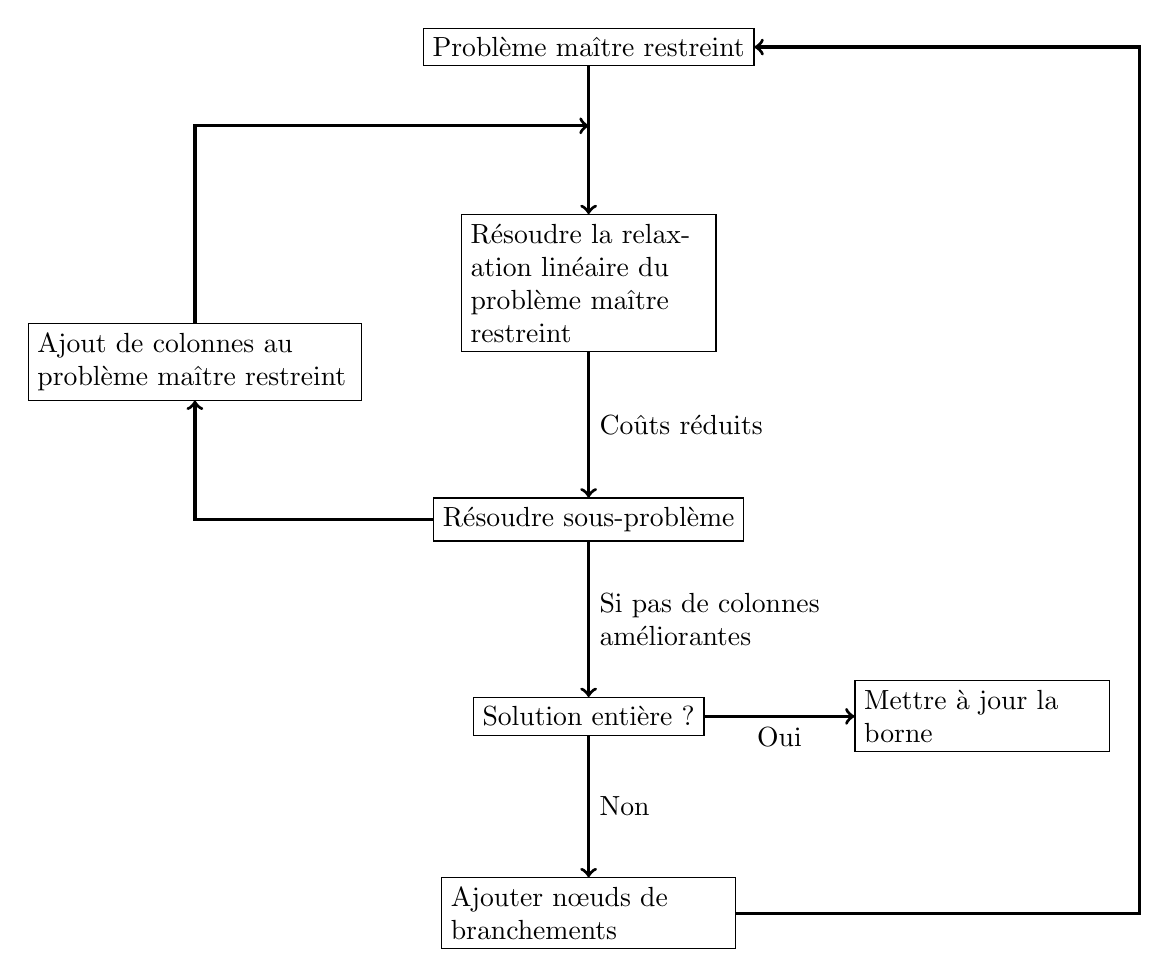
\begin{tikzpicture}

\node[draw,rectangle] (0) at (5,6) {Problème maître restreint};

\node[draw,rectangle,text width=3cm] (1) at (5,3) {Résoudre la relaxation linéaire du problème maître restreint};

\node[draw,rectangle] (2) at (5,0) {Résoudre sous-problème};

\node[draw,rectangle,text width=4cm] (3) at (0,2) {Ajout de colonnes au problème maître restreint};

\node[draw,rectangle] (4) at (5,-2.5) {Solution entière ?};

\node[draw,rectangle,text width=3cm] (5) at (10,-2.5) {Mettre à jour la borne};

\node[draw,rectangle,text width=3.5cm] (6) at (5,-5) {Ajouter nœuds de branchements};

\draw[->,very thick] (0)--(1);
\draw[->,very thick] (1)--(2)node[right,midway]{Coûts réduits};
\draw[->,very thick] (2.west)-|(3.south);
\draw[->,very thick] (3.north)|-(5,5);
\draw[->,very thick] (2)--(4)node[text width=3.5cm,right,midway]{Si pas de colonnes améliorantes};
\draw[->,very thick] (4)--(5)node[midway,below]{Oui};
\draw[->,very thick] (4)--(6)node[midway,right]{Non};
\draw[->,very thick] (6.east)-|(12,-3)|-(0.east);

\end{tikzpicture}
\caption{Figure illustrant le branch and price.\label{fig:BP}}
\end{figure}


\subsection{Les stratégies de branchements}

Pour les stratégies de branchements nous nous sommes inspirés des stratégies présentées dans l'article de Feillet et al. \cite{feillet2010}.
Il présente deux stratégies de branchement : nous appellerons la première : stratégie standard et la seconde : stratégie naturelle.

La stratégie standard correspond au branchement sur les variables de décision du RMP : $\schevar{s}{p}$.
On l'appelle stratégie standard car en général les arbres de branchement utilisent les variables de décisions du programme linéaire associé.

Lorsque la variable $\schevar{s}{p}$ est contrainte à 1 il suffit de sélectionner cette tournée dans le RMP et il faut supprimer tous les sommets présents dans cette tournée dans le PSP.

Cependant lorsqu'elle est contrainte à 0 la tournée n'est pas sélectionnée dans le RMP ($\schevar{s}{p}=0$) et dans le PSP il faut trouver des tournées différentes de cette tournée.
Ce qui implique de calculer les deux meilleurs plus court chemins et plus généralement les $d$ meilleurs plus court chemins lorsqu'il y a $d$ tournées contraintes à 0.

Ce branchement est peu efficace car il ne limite que très peu l'espace de recherche du PSP et du RMP. 
Alors que le branchement avec la variable $\schevar{s}{p}=1$ est plus fort car il permet de se rapprocher d'une solution entière assez rapidement.

La stratégie naturelle correspond au branchement sur les variables de flots $x_{ij}$.
Nous rappelons que $x_{ij}$ indique si la tâche $j$ est effectuée après la tâche $i$.
Cette stratégie est plus naturelle car elle branche sur les variables qui sont connectées à nos tournées.
Ces variables représentent les décisions locales prises par les véhicules.
Cette stratégie est devenue une norme pour les problèmes de tournées de véhicules.
Notons $f_{ij}$ le flot sur l'arc $(i,j)$.
Pour le branchement on choisit un arc $(i,j)$ tel que $0<f_{ij}<1$ ($f_{ij}=\sumP{p} x_{ij}^p$).
Dans ce cas deux branches sont dérivées :
\begin{itemize}
\item Dans une branche, l'arc ne doit pas appartenir à la solution : $f_{ij}=0$.
\item Dans l'autre branche, l'arc doit appartenir à la solution $f_{ij}=1$.
\end{itemize}

Si $f_{ij}$ est contraint à 1 alors dans le PSP les arcs $(i,k),~\forall k\not=j$ et  $(k,j),~\forall k\not=i$ doivent être supprimés.
Toutes les tournées générées passeront soit par l'arc $(i,j)$, soit ne passeront ni par $i$ ni par $j$ car c'est le seul arc sortant pour $i$ et entrant pour $j$.
Dans le RMP, il faut supprimer toutes les tournées telles que : les tournées passent par un des arcs $(i,k),~\forall k\not=j$ et  $(k,j),~\forall k\not=i$.
De plus il faut forcer les tâches $i$ et $j$ à être exécutées : $\gamma_i=0$ et $\gamma_j=0$.
Les tâches $i$ et $j$ appartiennent forcément à la solution et comme tous les autres arcs ont été supprimés : $i$ est directement suivit de $j$ (l'arc $(i,j)$ appartient aussi à la solution).

Si $f_{ij}$ est contraint à 0 alors dans le PSP l'arc $(i,j)$ est supprimé. 
Aucune tournée générée avec le PSP ne contiendra l'arc $(i,j)$.
Dans le RMP, il faut supprimer toutes les tournées passant par l'arc $(i,j)$.
Ainsi $f_{ij}=0$ car aucune tournée ne passera par $j$ directement après $i$.

Ce branchement se base sur le fait que les tournées appartenant à une solution réalisable sont disjointes.
Dans le graphe représentant les tournées, tous les sommets (tâches) ont un degré deux.
Ainsi le flot sur un arc pour toute tournée est $0< f_{ij}<1$.
Cependant si les tâches peuvent être visitées plusieurs fois dans les solutions optimales alors cette stratégie de branchement est difficilement transposable car brancher sur certains arcs couperait des solutions optimales.


Il existe cependant d'autres stratégies de branchement comme par exemple la stratégie de branchement sur les fenêtres temporelles ou sur les contraintes de précédence.
Nous n'avons pas décidé d'implémenter ces stratégies car dans les instances que nous traitons il y a peu de contraintes de précédence. 
La stratégie sur les fenêtres temporelles nous semble peu efficace sur nos instances car le fait qu'il y ait plusieurs fenêtres temporelles fait qu'un branchement sur celles-ci ne converge que très peu vers une solution réalisable.


\subsection{Les stratégies de parcours de l'arbre de branchements}

L'arbre de branchements représente l'espace des solutions.
Son parcours est donc très important pour obtenir la solution optimale avec le moins de temps possible.
Il existe différentes stratégies de recherche dans un arbre parcours : parcours en profondeur (depth-first search en anglais), parcours en largeur (breadth-first search en anglais) et parcours du "meilleur d'abord" (best-first search en anglais).

Le parcours en profondeur vise à obtenir une solution entière rapidement, puis parcours l'arbre pour essayer d'améliorer cette solution entière.
Le n\oe ud le plus profond dans l'arbre est sélectionné en premier.
Comme cette solution donne une borne, cette stratégie permet de couper de nombreuses branches.

Le parcours en largeur permet de parcourir l'arbre dans sa totalité niveau par niveau. 
La racine étant au niveau 0, ses voisins au niveau 1 et ainsi de suite ...
Cette stratégie n'est pas efficace car elle demande de stocker en mémoire tous les n\oe uds d'un niveau de l'arbre.

Le parcours "meilleur d'abord" permet d'obtenir une solution entière de bonne qualité, il est même probable que cette solution soit optimale.
Le n\oe ud avec la meilleure solution relâchée est sélectionné en premier.
Jusqu'à l'obtention de cette solution aucune branche ne sera coupée.
Cependant lorsque cette solution est trouvée la plupart des branches seront coupées.

Il est aussi possible de coupler certain parcours entre eux comme par exemple : le parcours en profondeur et le parcours "meilleur d'abord" : les n\oe uds les plus profonds dans l'arbre sont gardés puis celui qui à la meilleure solution relâchée est sélectionné.






%%%%%%%%%%%%%%%%%%%%%%%%%%%%%%%%%%%%%%%
%%%%%%%%%%%%%%%%%%%%%%%%%%%%%%%%%%%%%%%